\documentclass[aspectratio=169]{beamer}\usepackage[utf8]{inputenc}\usepackage[T1]{fontenc}\usepackage[spanish]{babel}\usepackage{graphicx,booktabs}\usetheme{Madrid}\graphicspath{{../../../outputs/parte_2/14_segunda_pasada/figuras/}{../../../outputs/parte_2/13_figuras_finales/}}\title{Parte 2: concentraciones y composición}\subtitle{Cierre metodológico ampliado}\date{Septiembre de 2026}\begin{document}\frame{\titlepage}
\begin{frame}{Qué se mantuvo fijo}HDBSCAN: tamaño mínimo 10, muestras mínimas 20, EOM. Las variables económicas se incorporan sólo después. La segunda pasada documenta y audita; no redefine membresías.\end{frame}
\begin{frame}{Exploración espacial}24 DBSCAN + 30 HDBSCAN + 3 OPTICS. Diagnósticos $k$-NN, KDE y hexágonos. Coordenadas UTM 14N en metros.\end{frame}
\begin{frame}[plain]\centering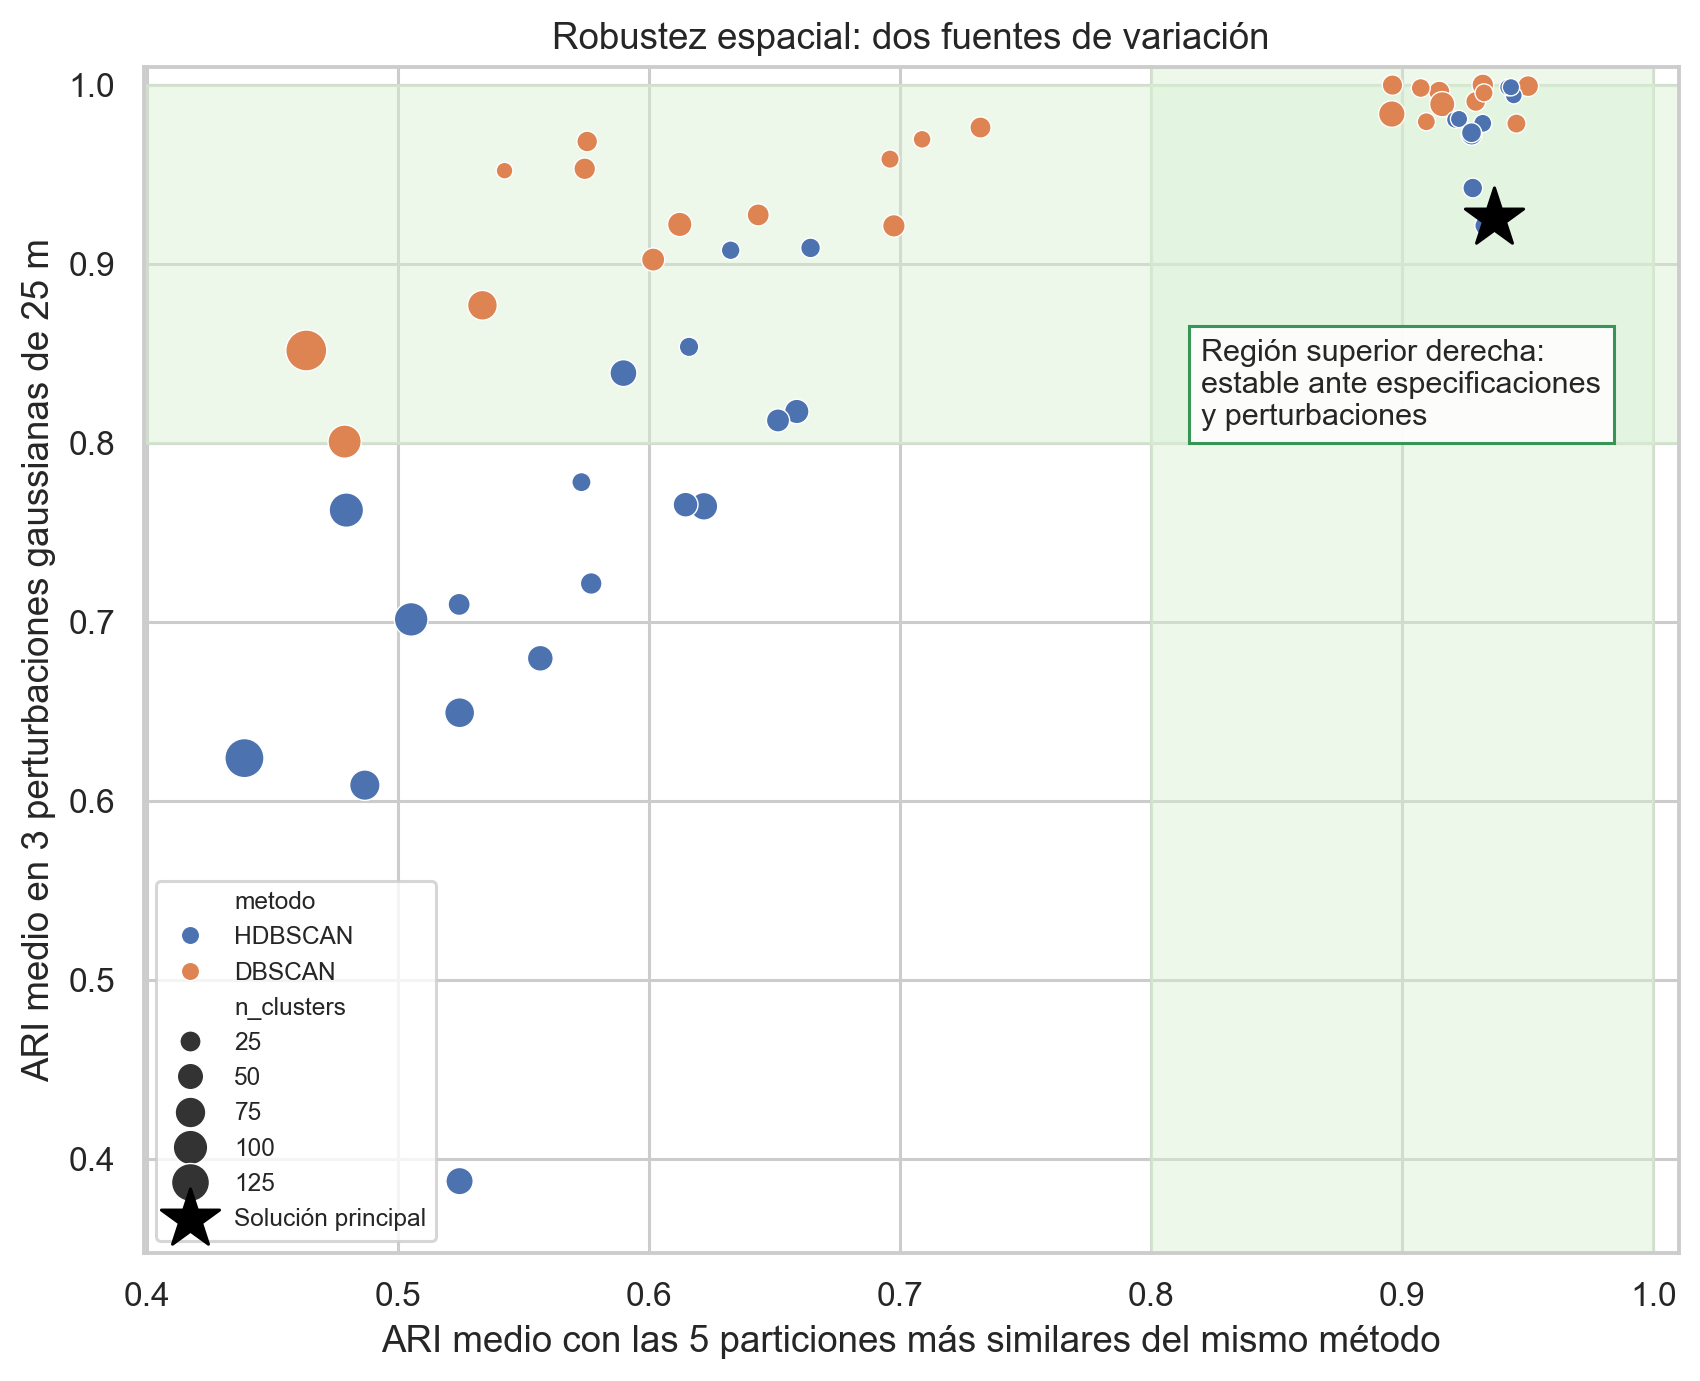
\includegraphics[width=.92\paperwidth,height=.9\paperheight,keepaspectratio]{01_robustez_ari_documentada.png}\end{frame}
\begin{frame}{Cómo leer ARI}ARI compara particiones completas y corrige acuerdo por azar. 1=idénticas; cerca de 0=azar. Es global: no dice qué cluster cambió. El eje X usa las cinco particiones del mismo método con mayor ARI, no vecindad paramétrica.\end{frame}
\begin{frame}{¿Domina el mega-cluster?}Top-5: ARI global 0.937; sin ruido 0.992; sin mega 0.819. Perturbación 25 m: 0.926, 0.986 y 0.896. La estabilidad sigue alta, pero el agregado global sí recibe aporte de grupos grandes.\end{frame}
\begin{frame}{ARI versus estabilidad individual}ARI compara toda la partición. Jaccard solapa dos clusters. Estabilidad de membresía cuenta en cuántas de cinco especificaciones conserva cada punto su cluster emparejado. No es cohesión ni persistencia nativa HDBSCAN.\end{frame}
\begin{frame}[plain]\centering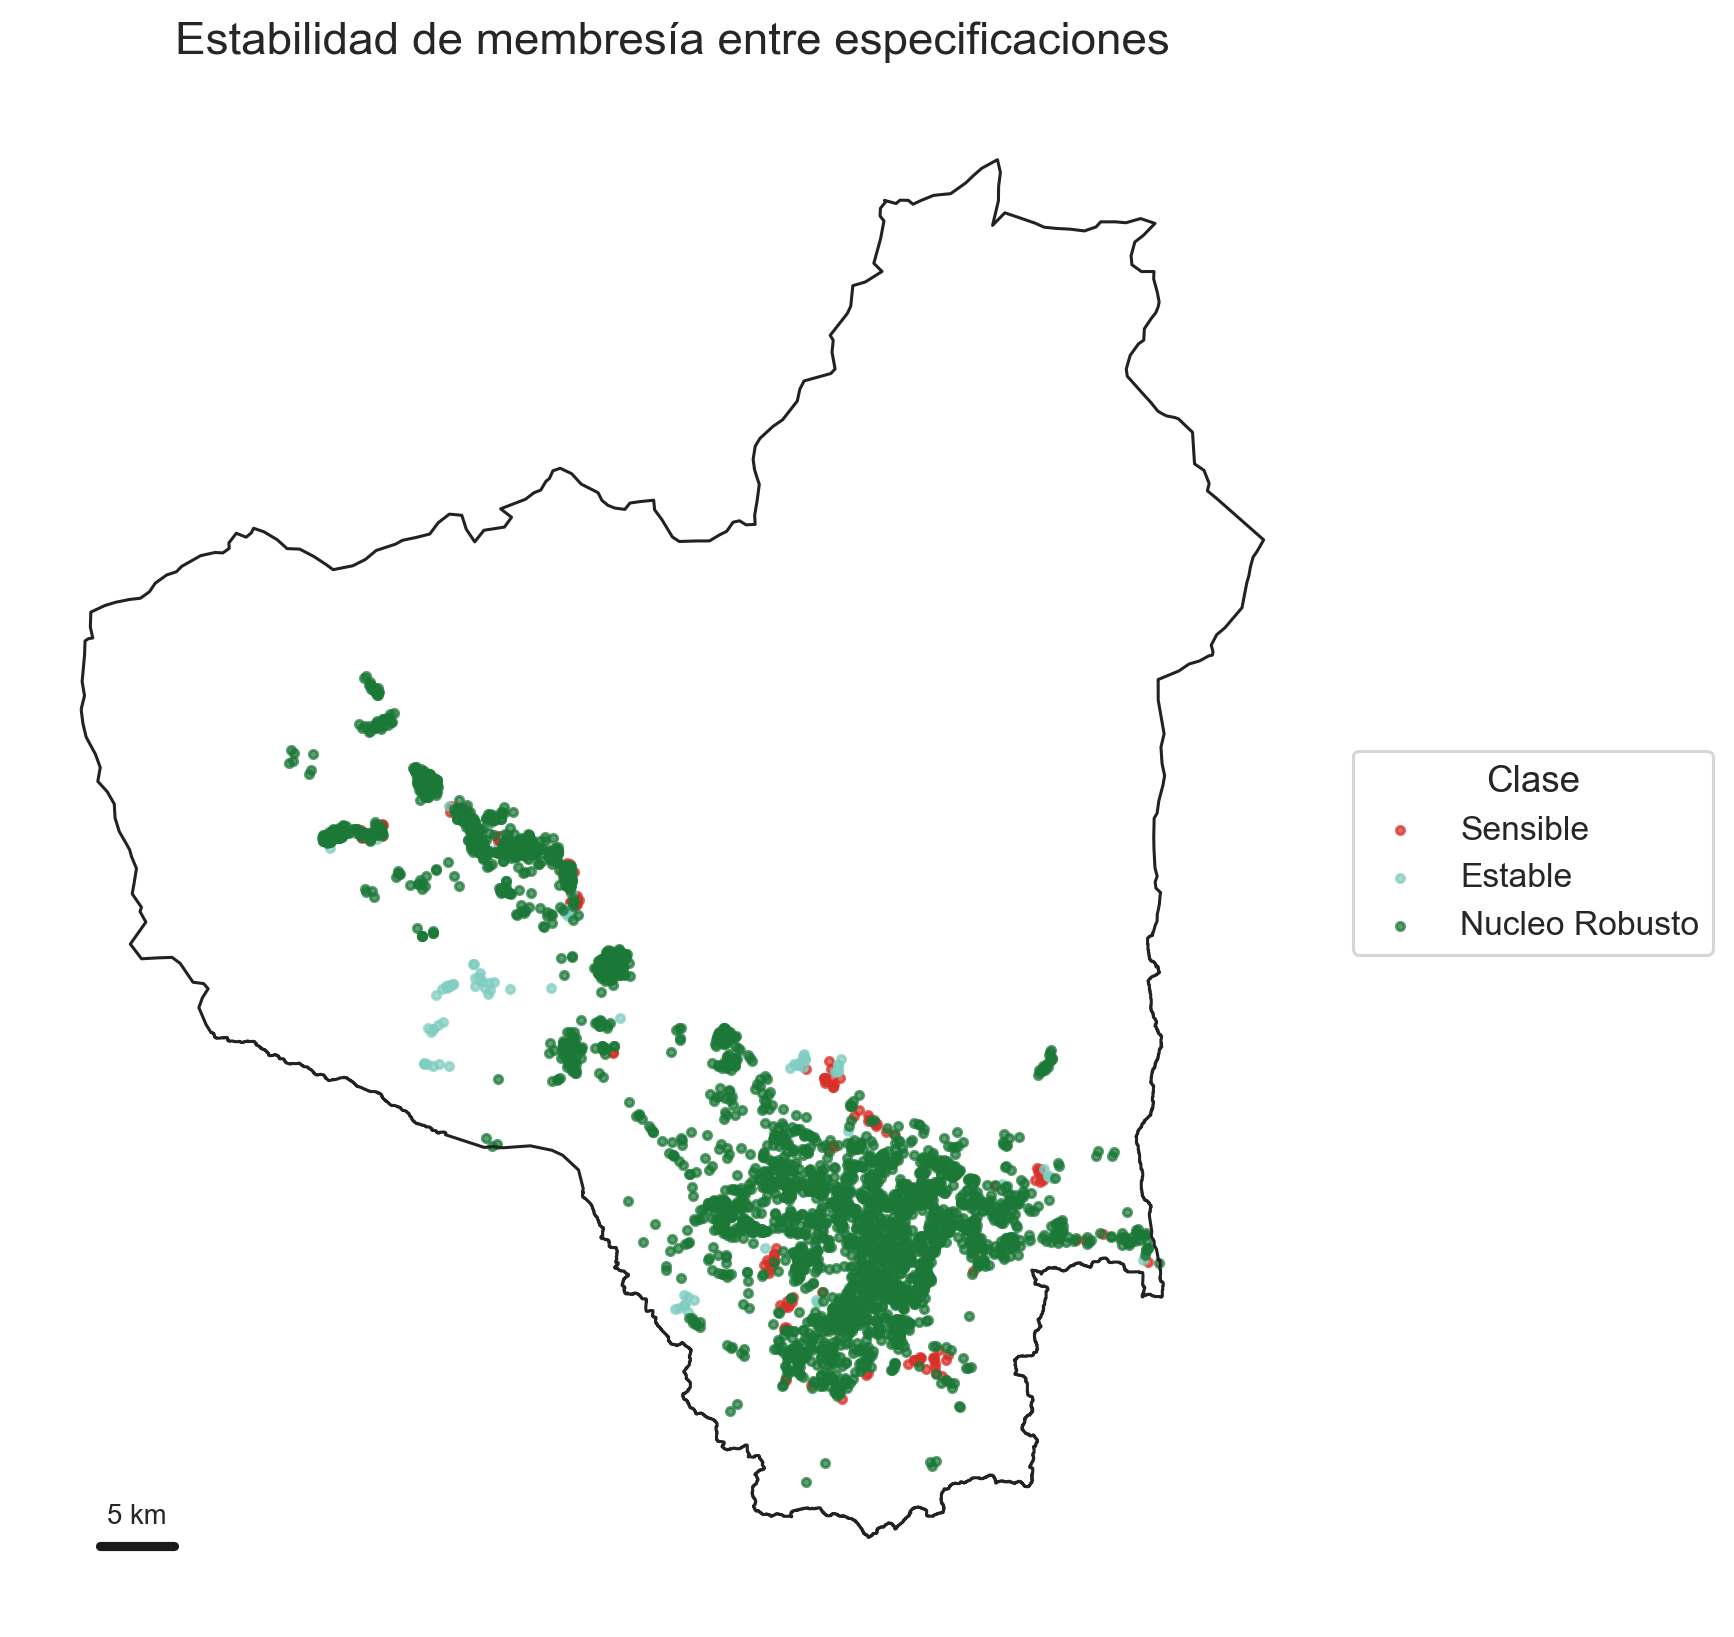
\includegraphics[height=.9\paperheight]{02_estabilidad_membresia.png}\end{frame}
\begin{frame}{Solución principal}22 clusters municipales; 18 dentro de cuenca; 578 puntos interiores dispersos. El cluster 20 reúne 1,997 establecimientos. Es referencia operativa, no geografía única.\end{frame}
\begin{frame}[plain]\centering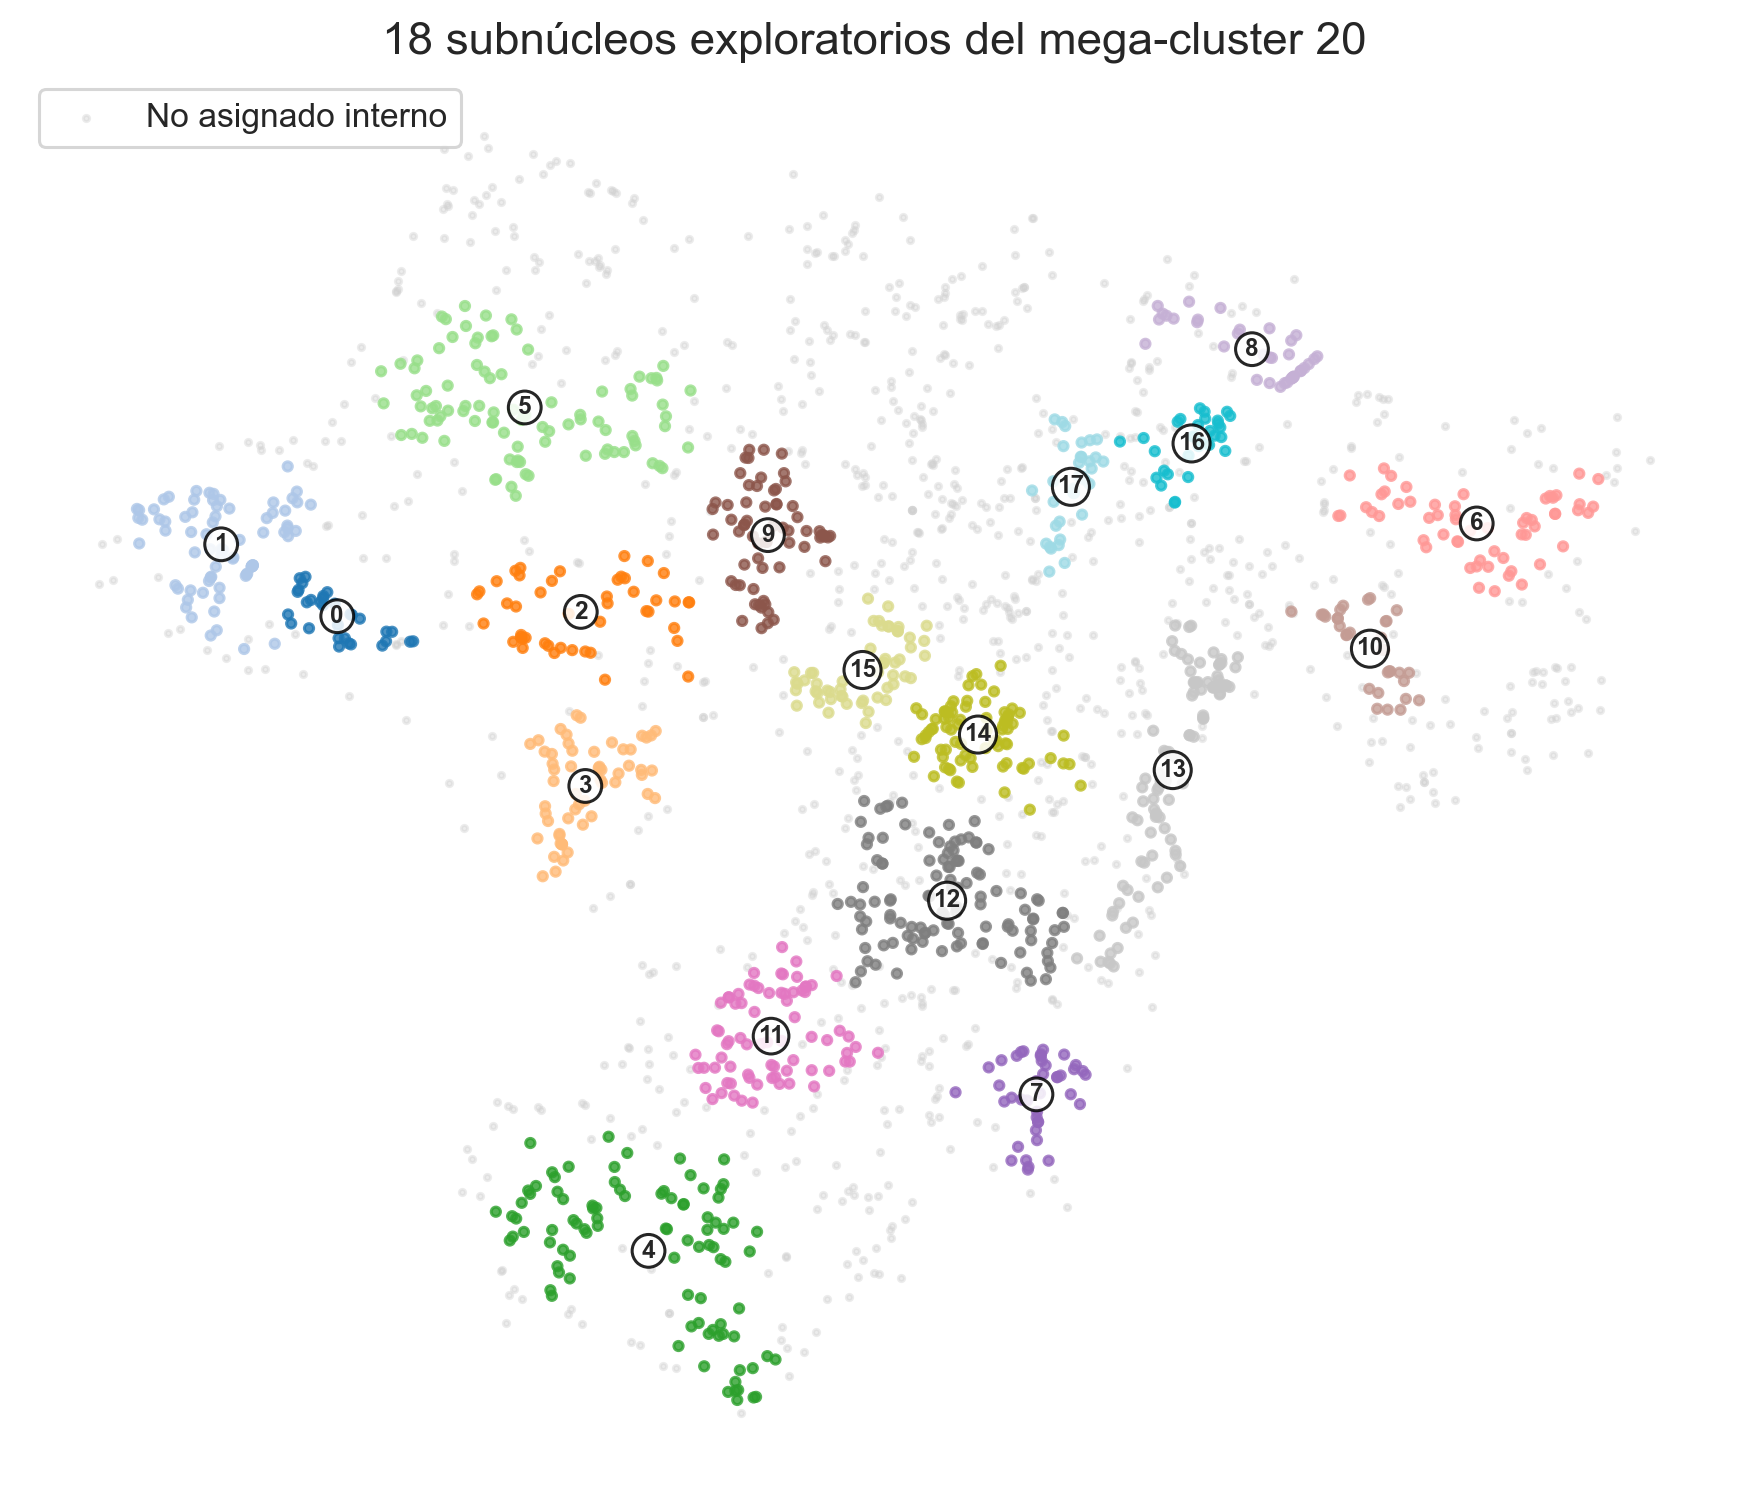
\includegraphics[height=.9\paperheight]{03_subnucleos_mega_etiquetados.png}\end{frame}
\begin{frame}{Mega-cluster: qué significa 44.5\% no asignado}HDBSCAN leaf, tamaño mínimo 30 y muestras mínimas 10, sólo coordenadas. Dieciocho ramas locales. Los no asignados carecen de densidad local suficiente en esta exploración, pero permanecen en el cluster 20 principal.\end{frame}
\begin{frame}[plain]\centering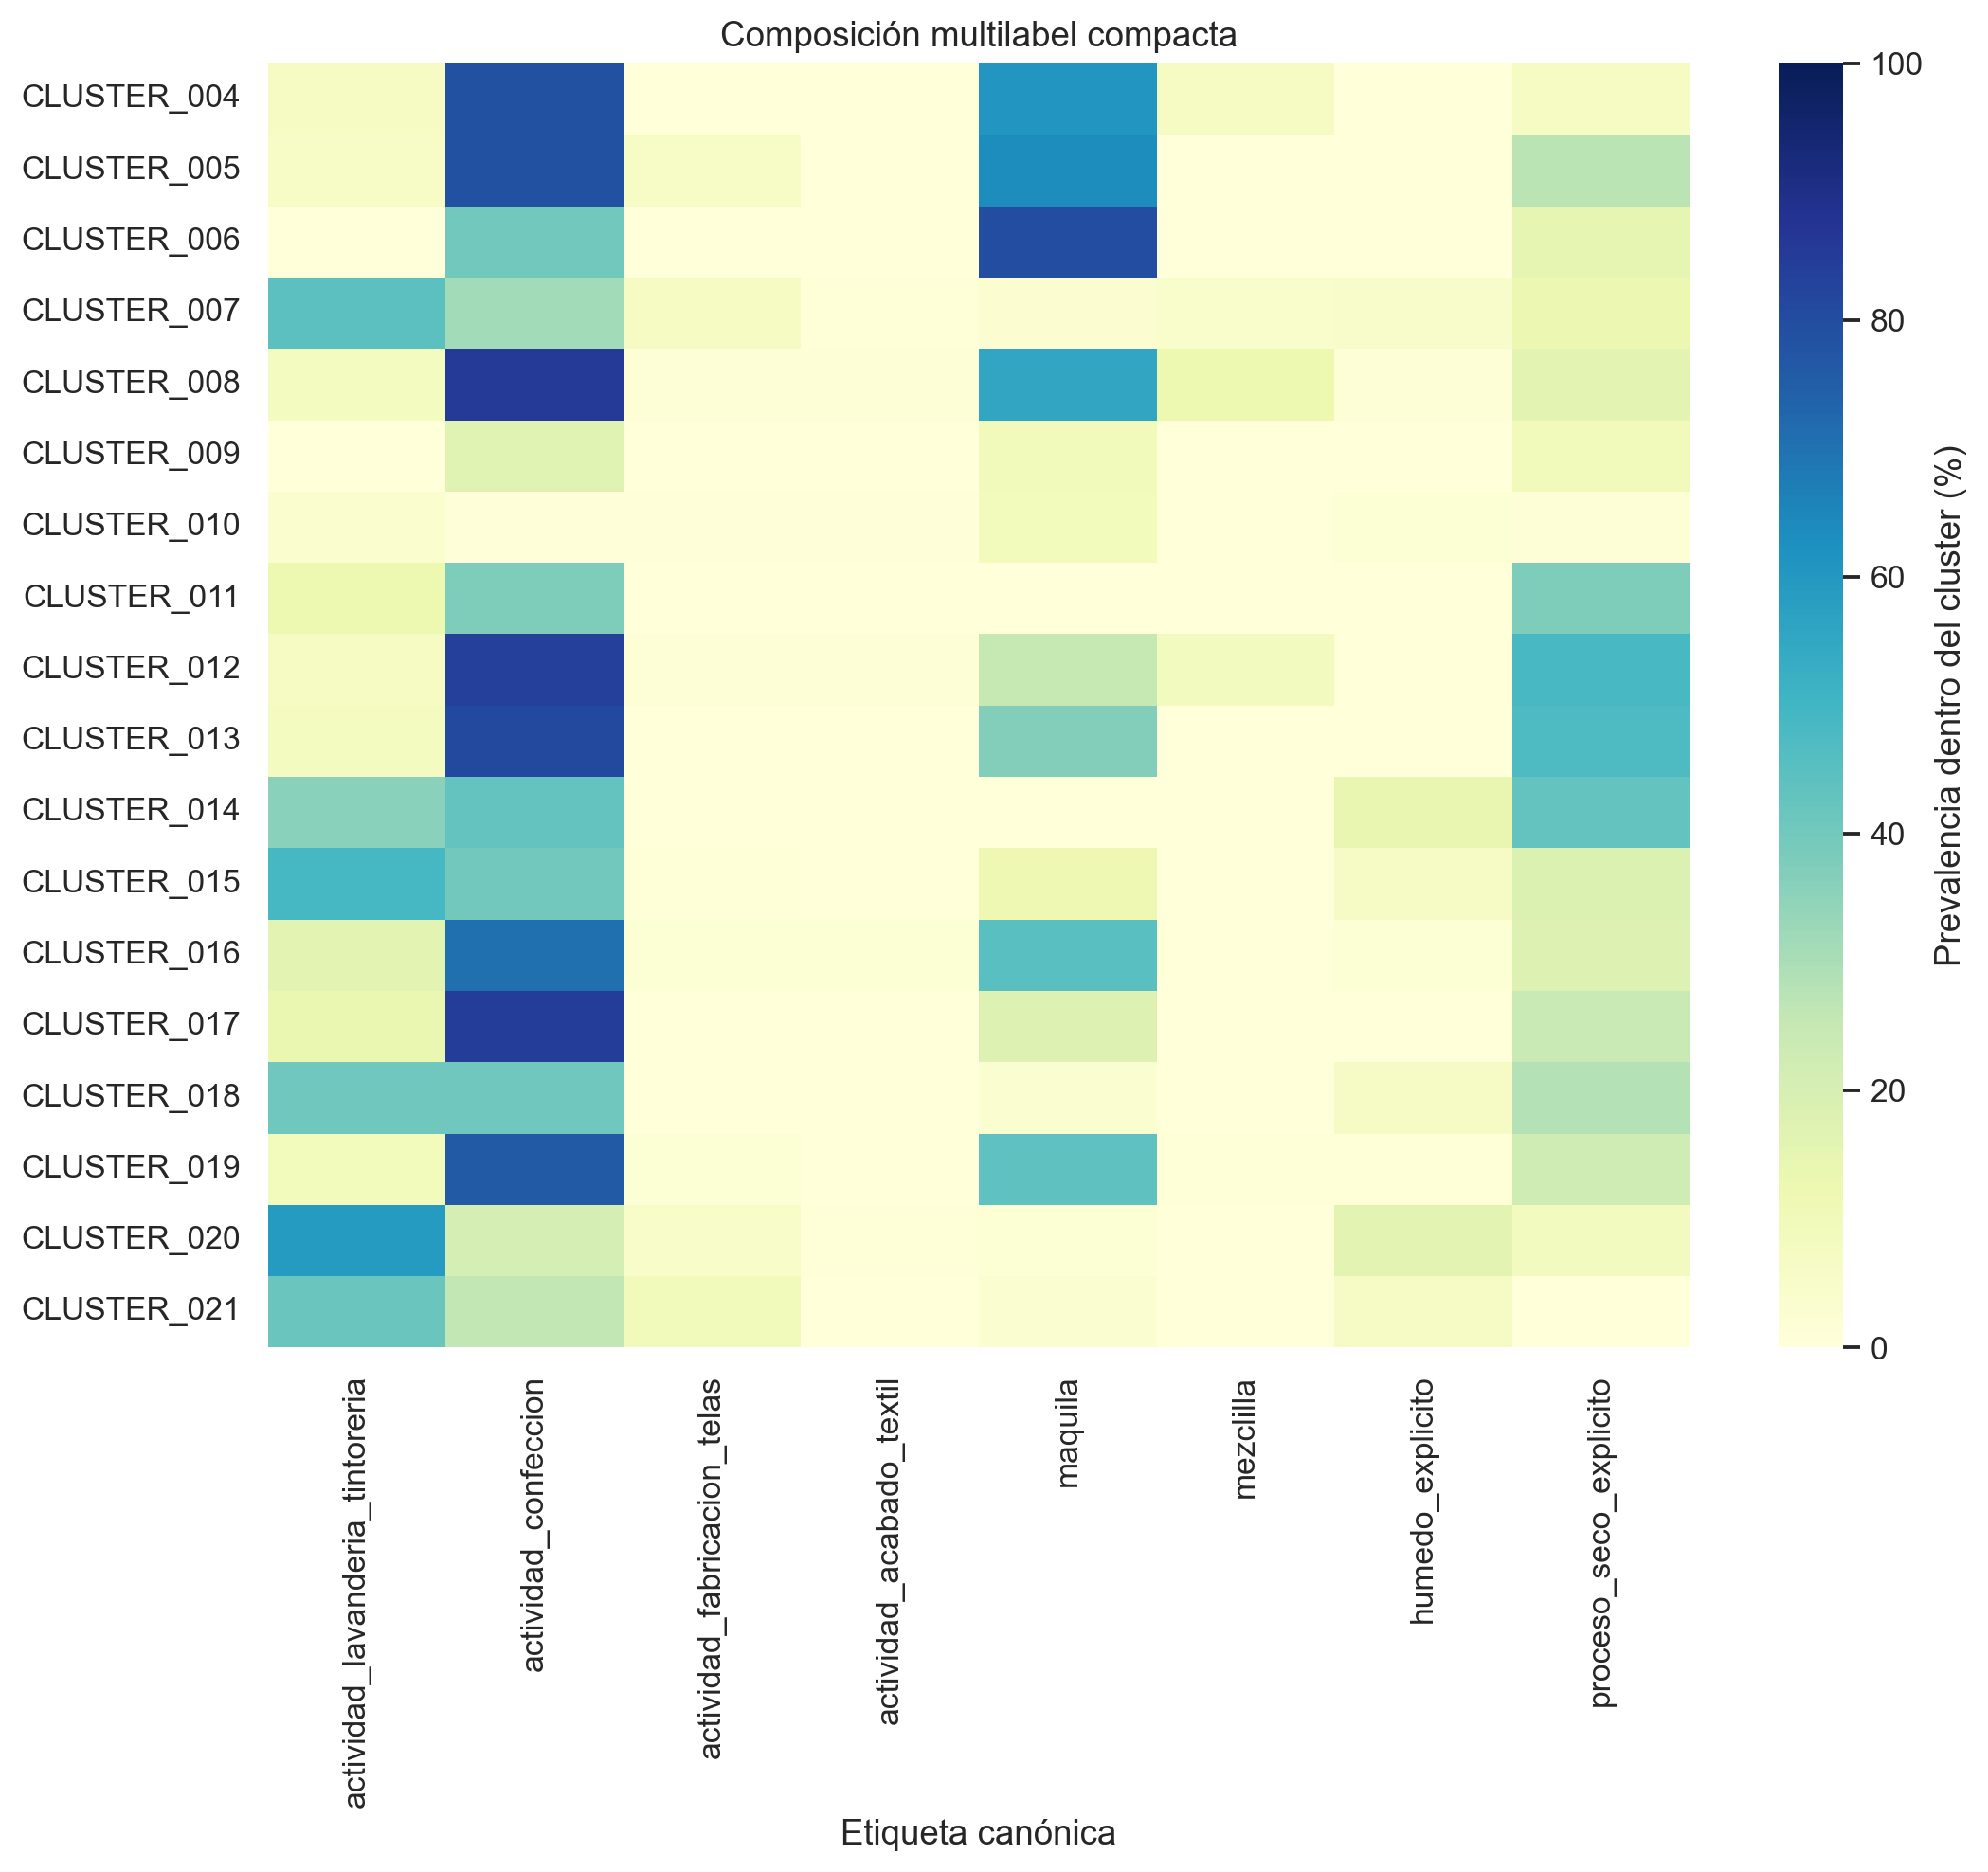
\includegraphics[height=.9\paperheight]{04_heatmap_compacto.png}\end{frame}
\begin{frame}{Por qué esas columnas}Ocho etiquetas centrales, interpretables y no excesivamente redundantes. Los términos crudos activan etiquetas canónicas; las reglas SCIAN forman categorías agregadas. El anexo y el HTML contienen las 18 señales útiles.\end{frame}
\begin{frame}[plain]\centering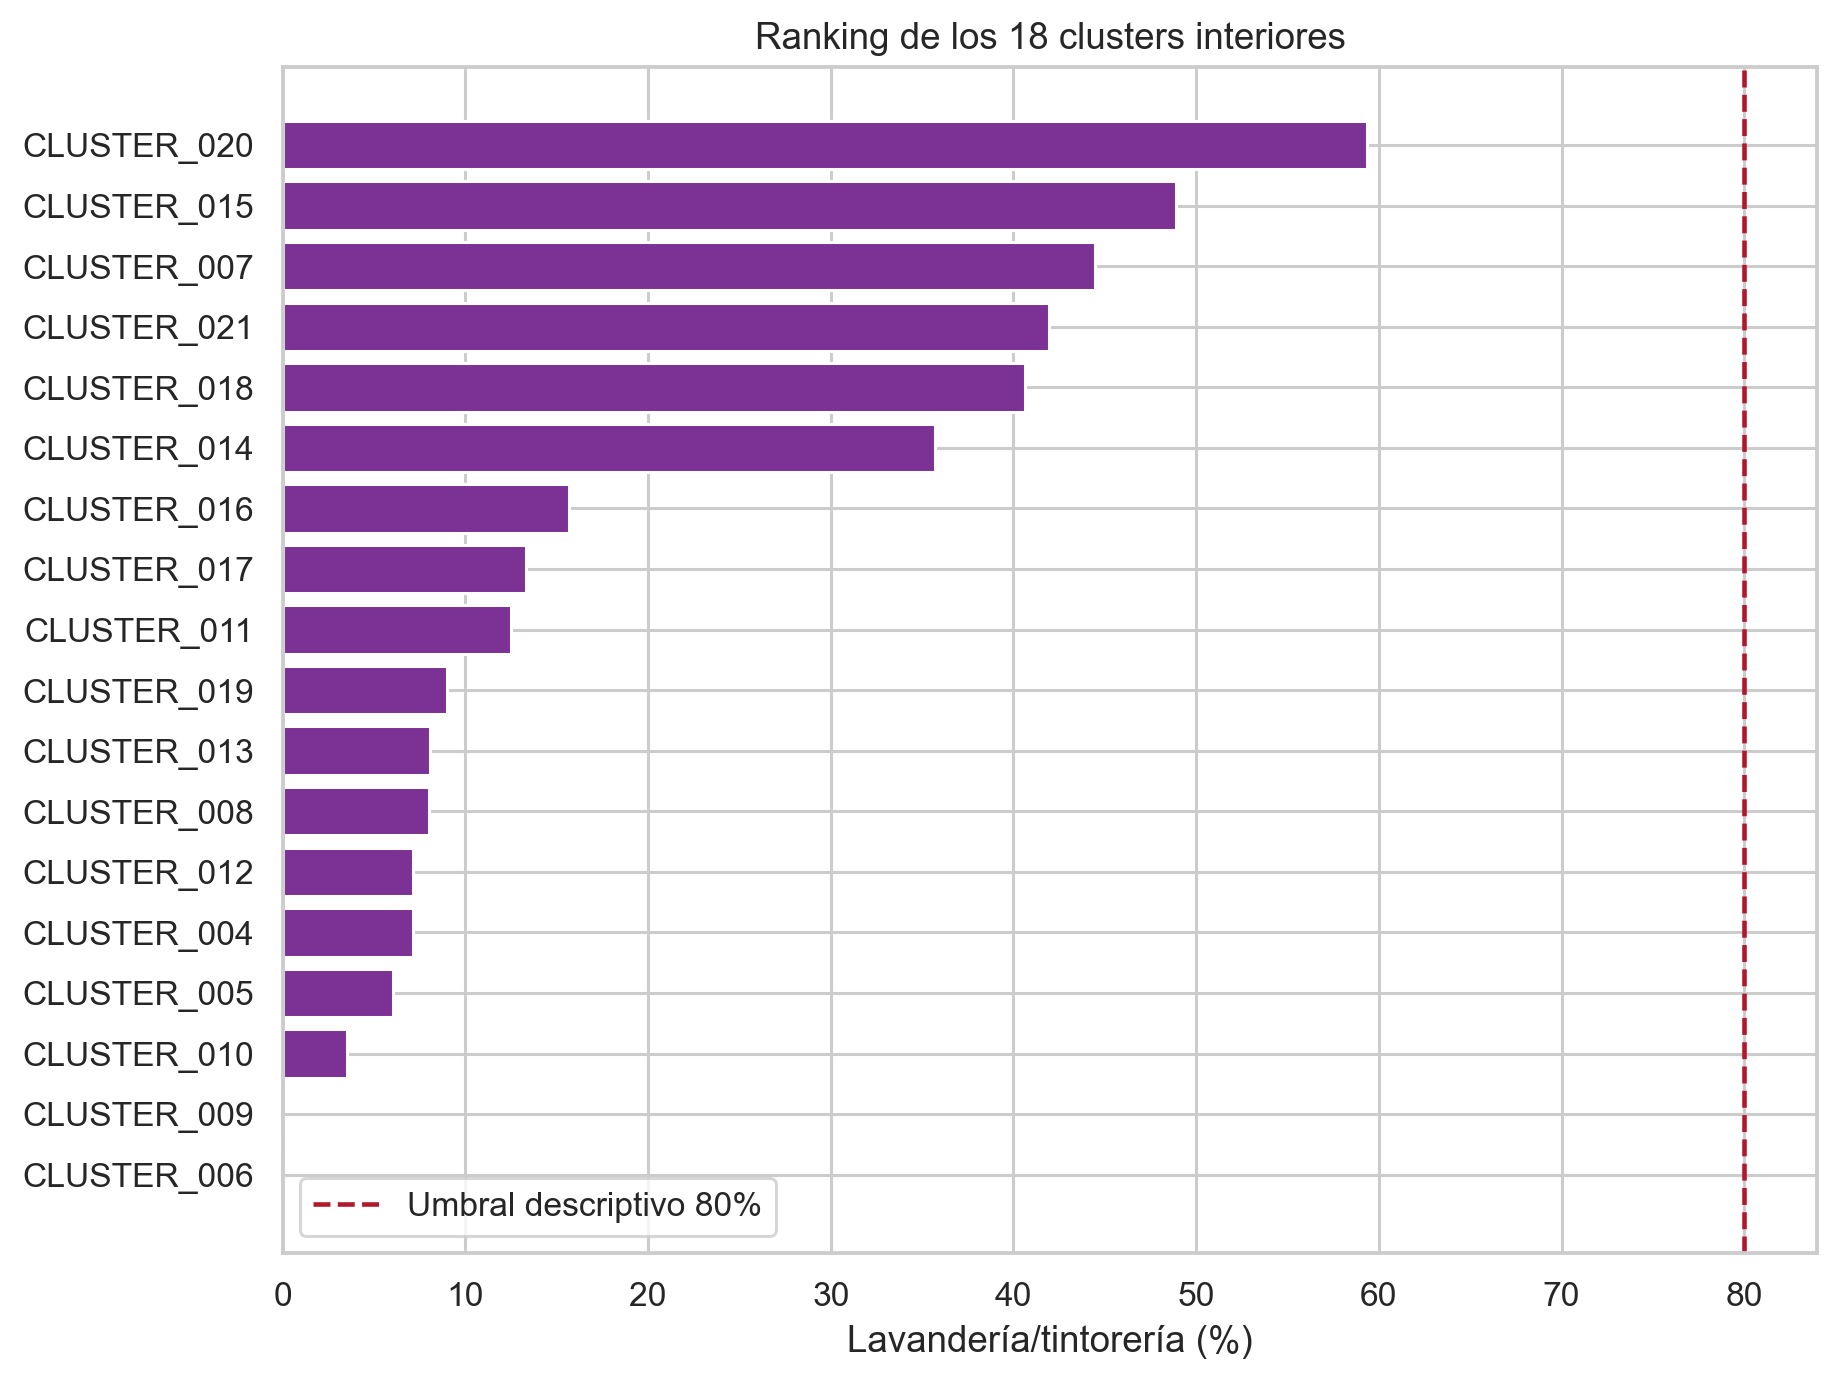
\includegraphics[height=.88\paperheight]{08_ranking_lavanderia.png}\end{frame}
\begin{frame}{Lavanderías y manufactura}12 concentraciones manufactureras, seis mixtas y ninguna con $\ge80\%$ lavandería. El 80\% es descriptivo. El patrón se conserva en seis escenarios; coexistencia no implica vínculo empresarial o hídrico.\end{frame}
\begin{frame}{Qué significa sobrerrepresentación}$lift=p_c/p_U$; $\log_2(lift)=0$ igualdad, positivo sobre-, negativo subrepresentación. Ejemplo: lift 2 significa prevalencia doble. Sólo se destaca con $n\ge5$, prevalencia $\ge5\%$, lift $\ge1.25$ y BH $\le.05$.\end{frame}
\begin{frame}[plain]\centering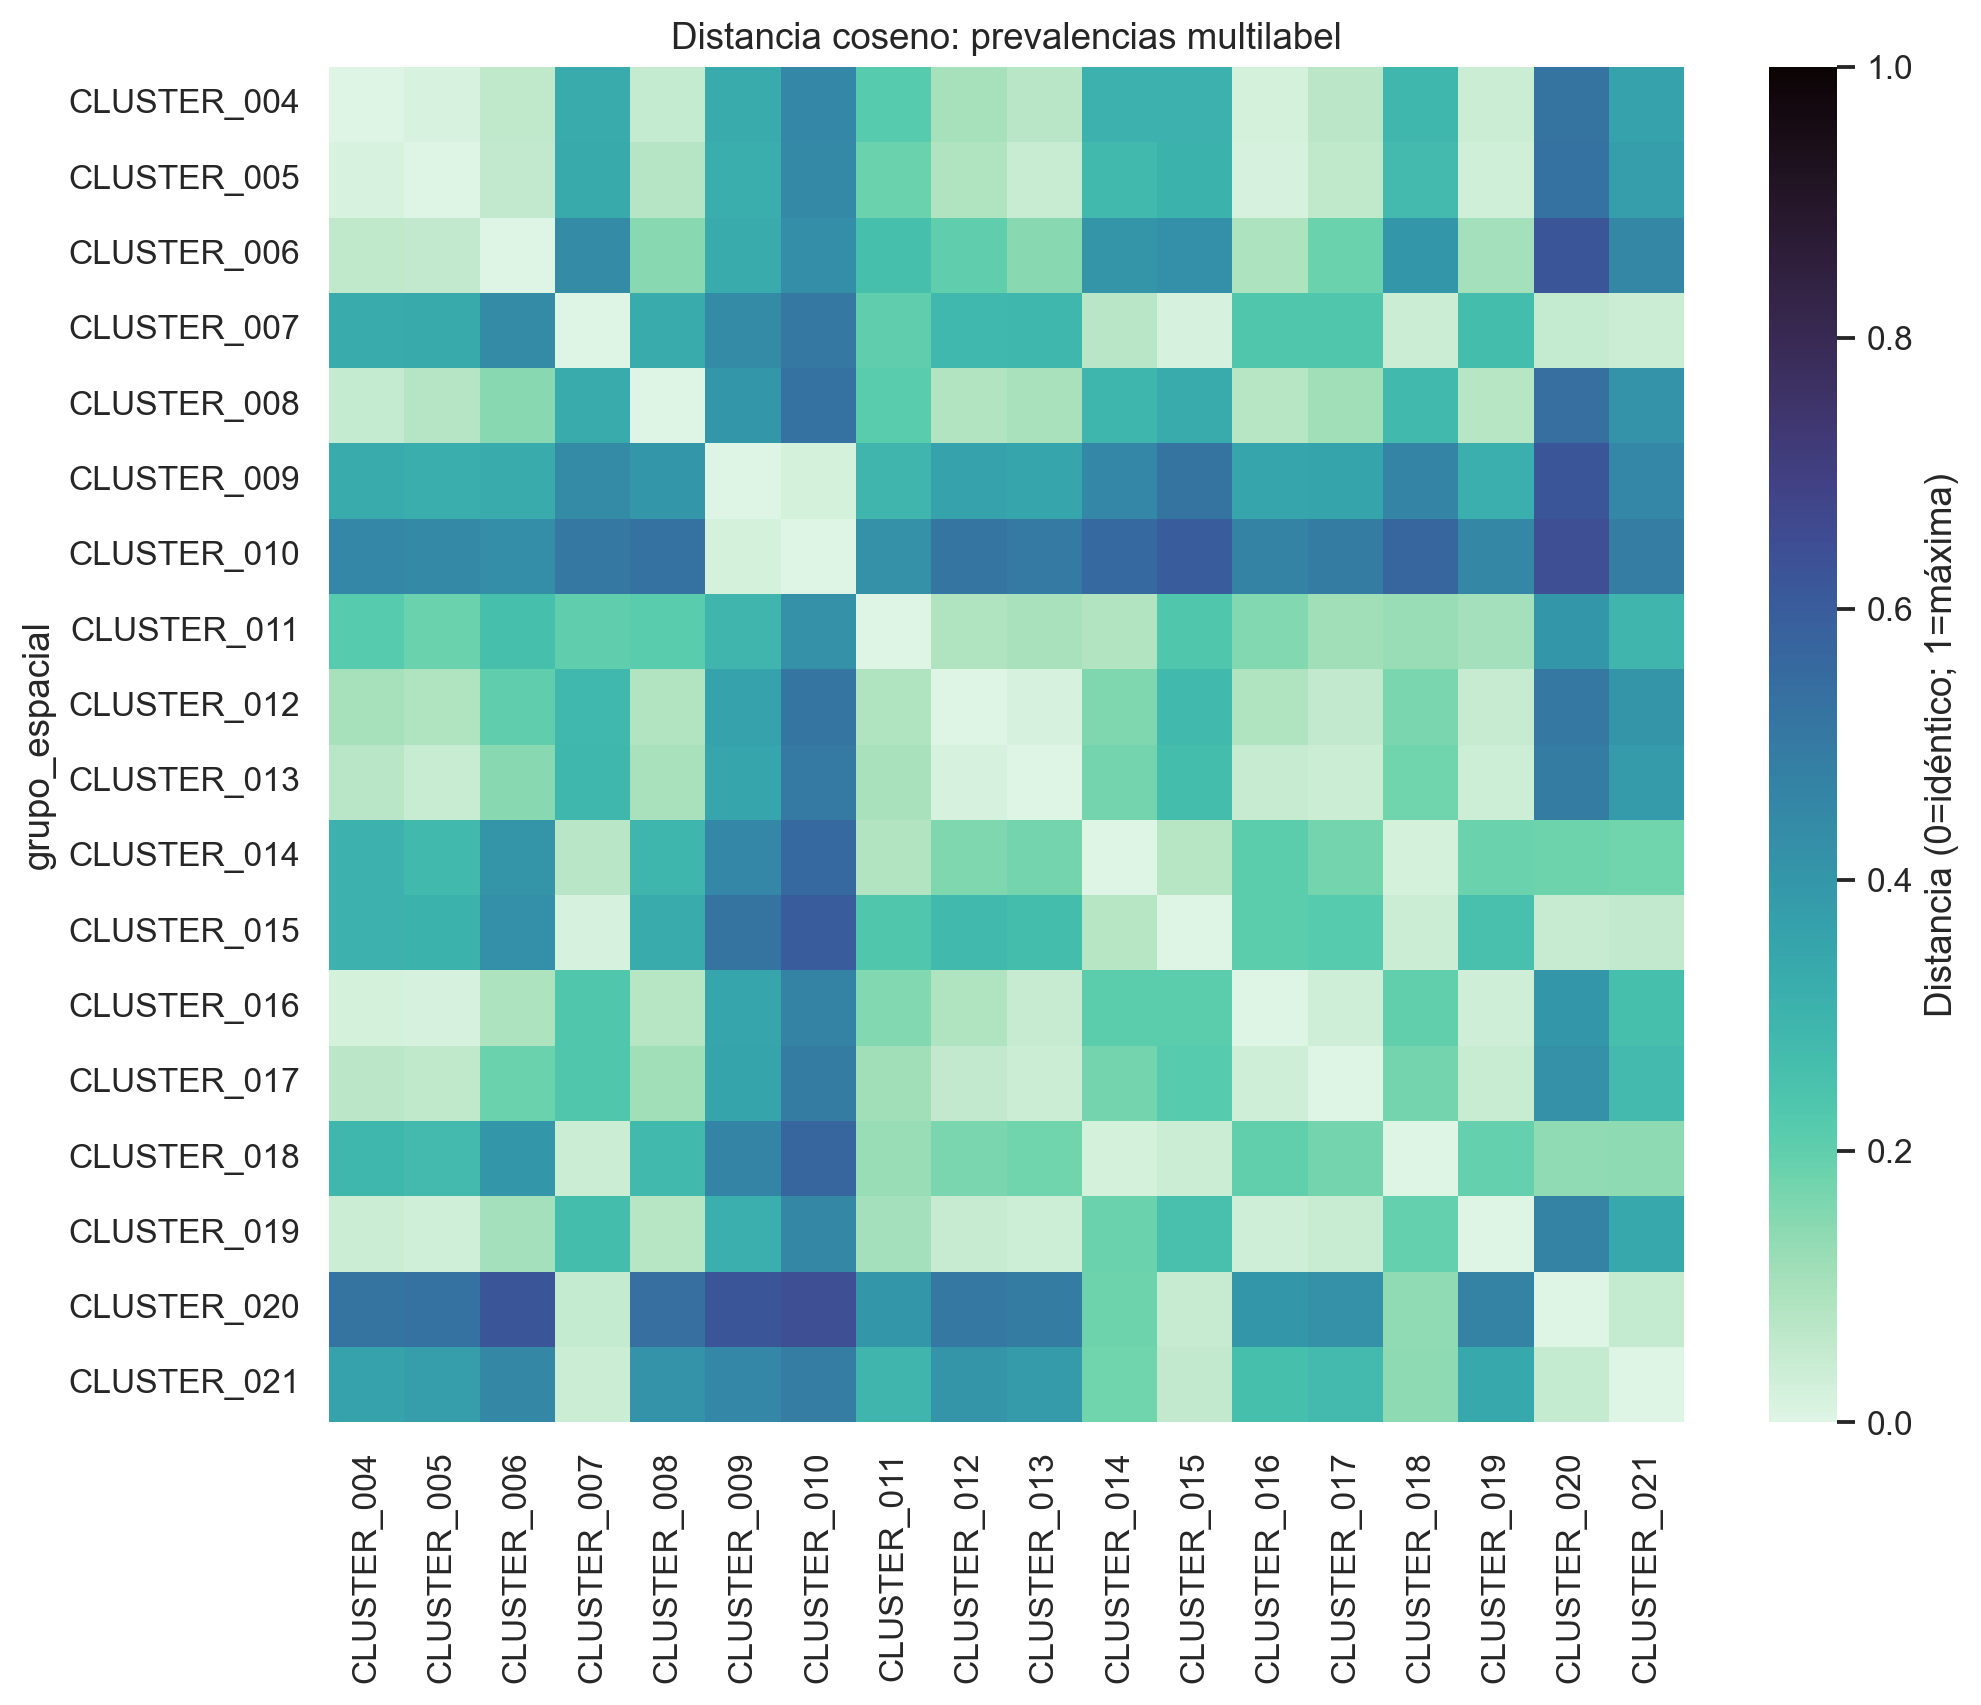
\includegraphics[height=.88\paperheight]{06_distancia_coseno_senales.png}\end{frame}
\begin{frame}[plain]\centering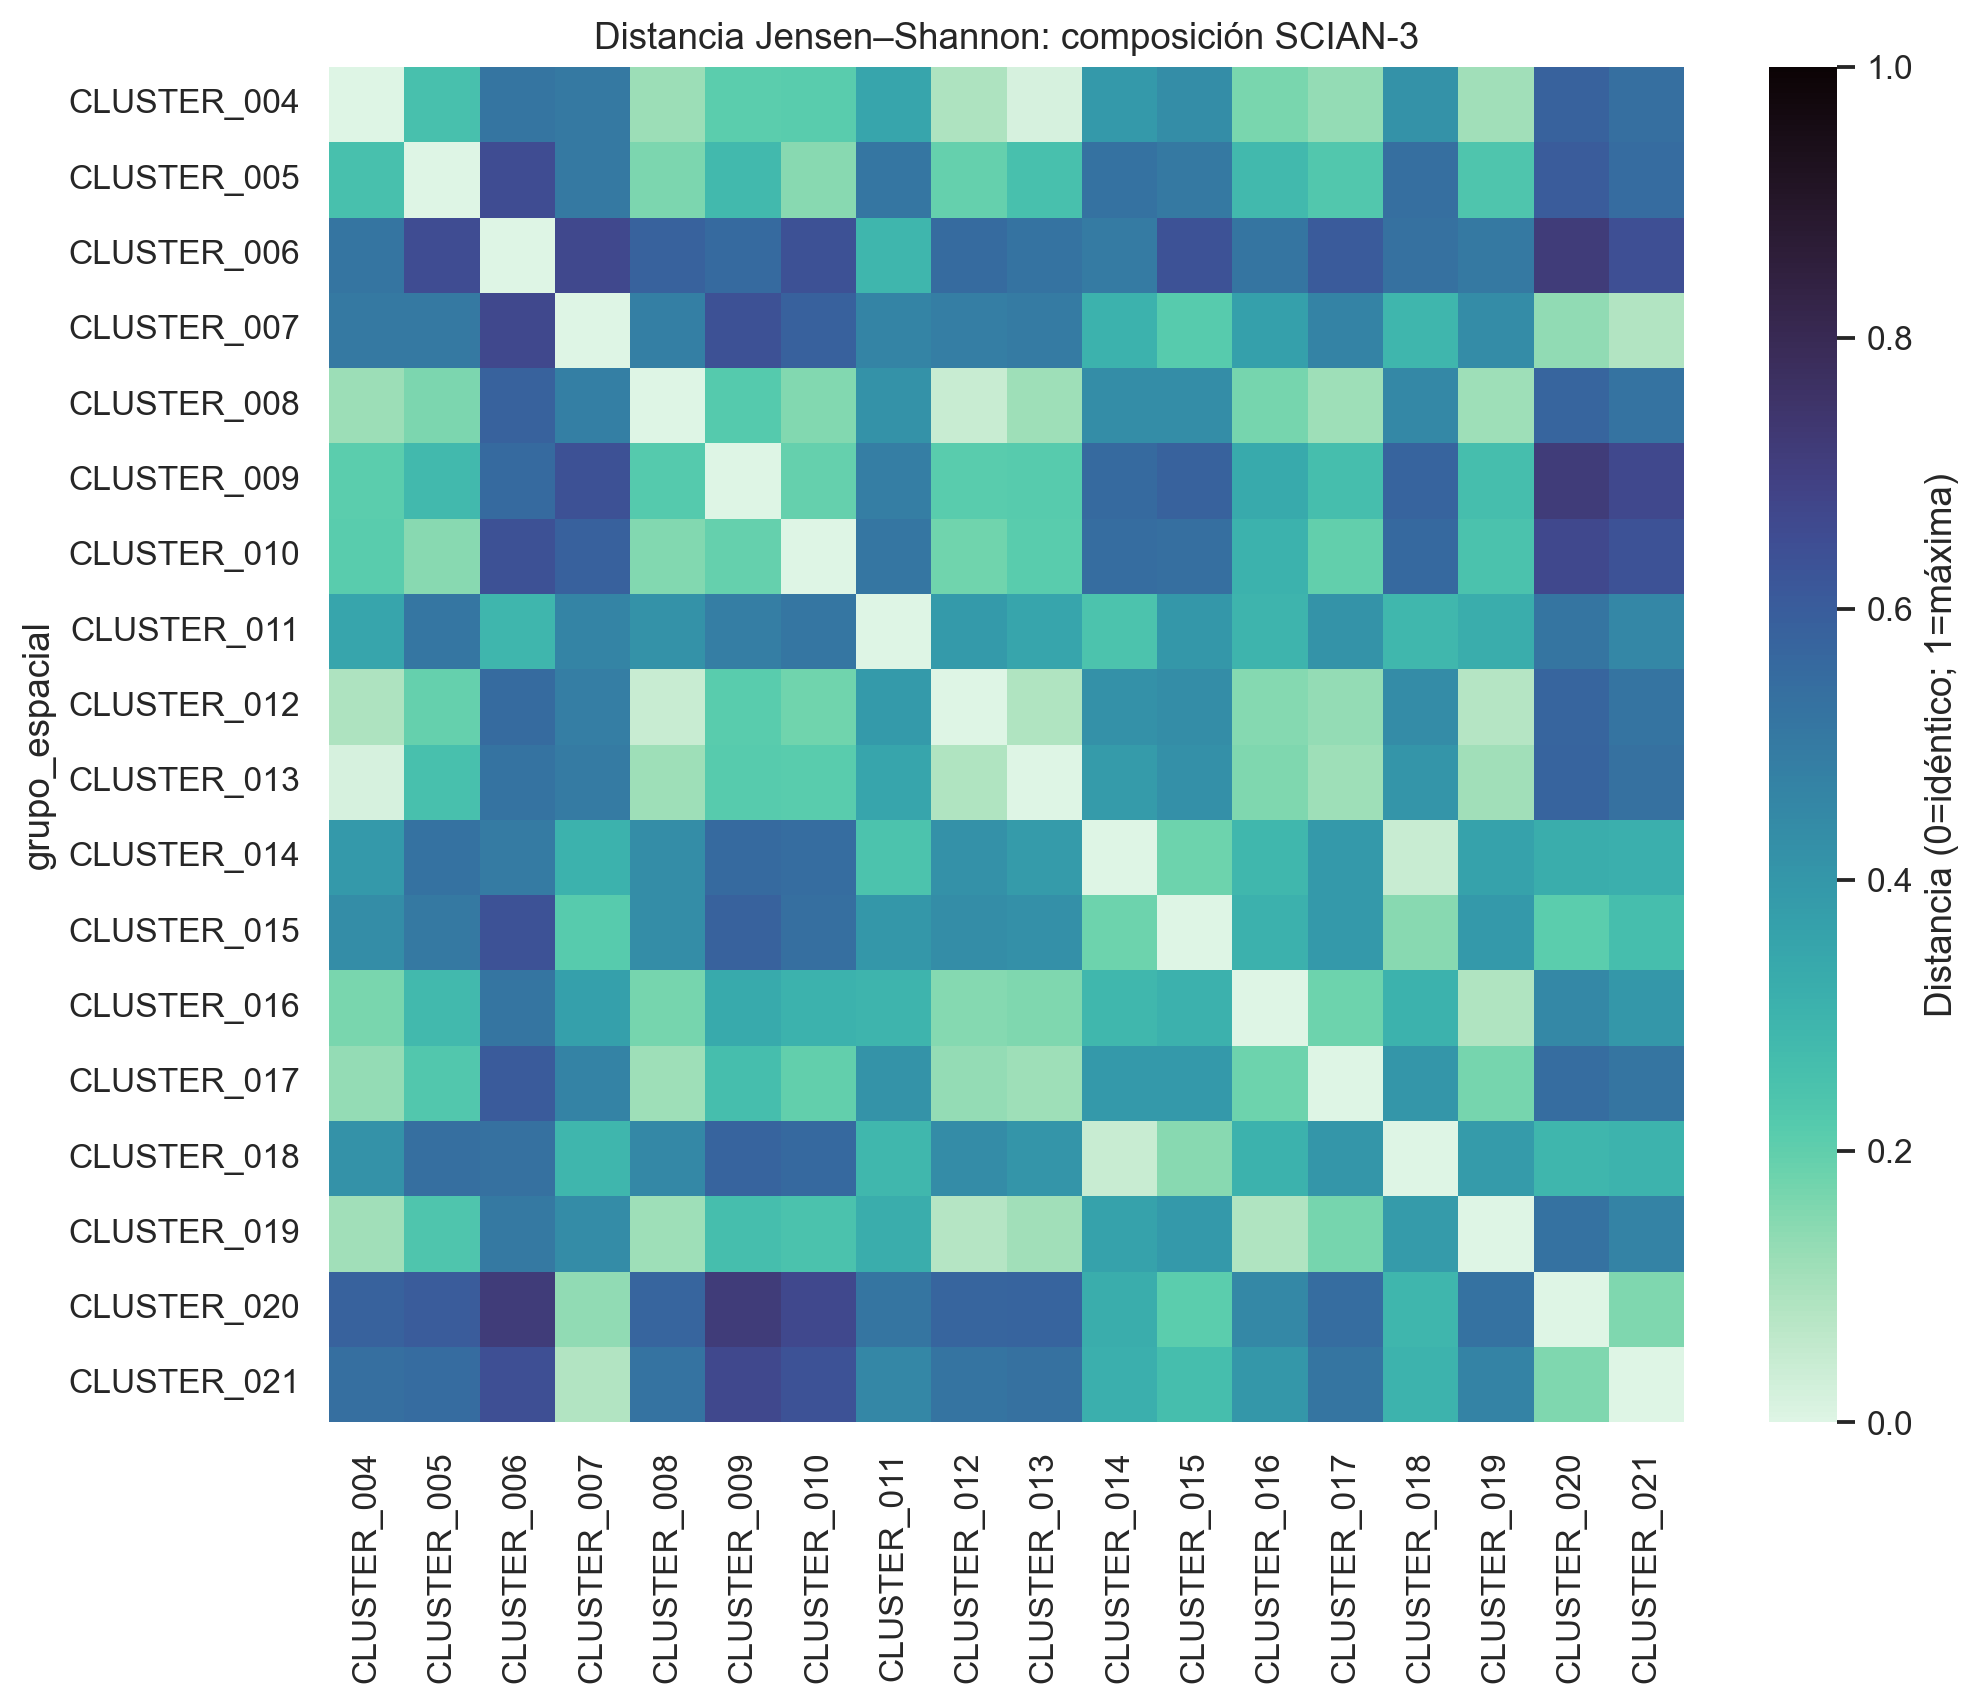
\includegraphics[height=.88\paperheight]{06_distancia_jensen_shannon_scian3.png}\end{frame}
\begin{frame}{Dos preguntas distintas}Coseno compara el patrón de prevalencias multilabel. Jensen--Shannon compara la distribución SCIAN-3. La tipología usa distancia combinada 50/50; valores bajos significan perfiles parecidos.\end{frame}
\begin{frame}[plain]\centering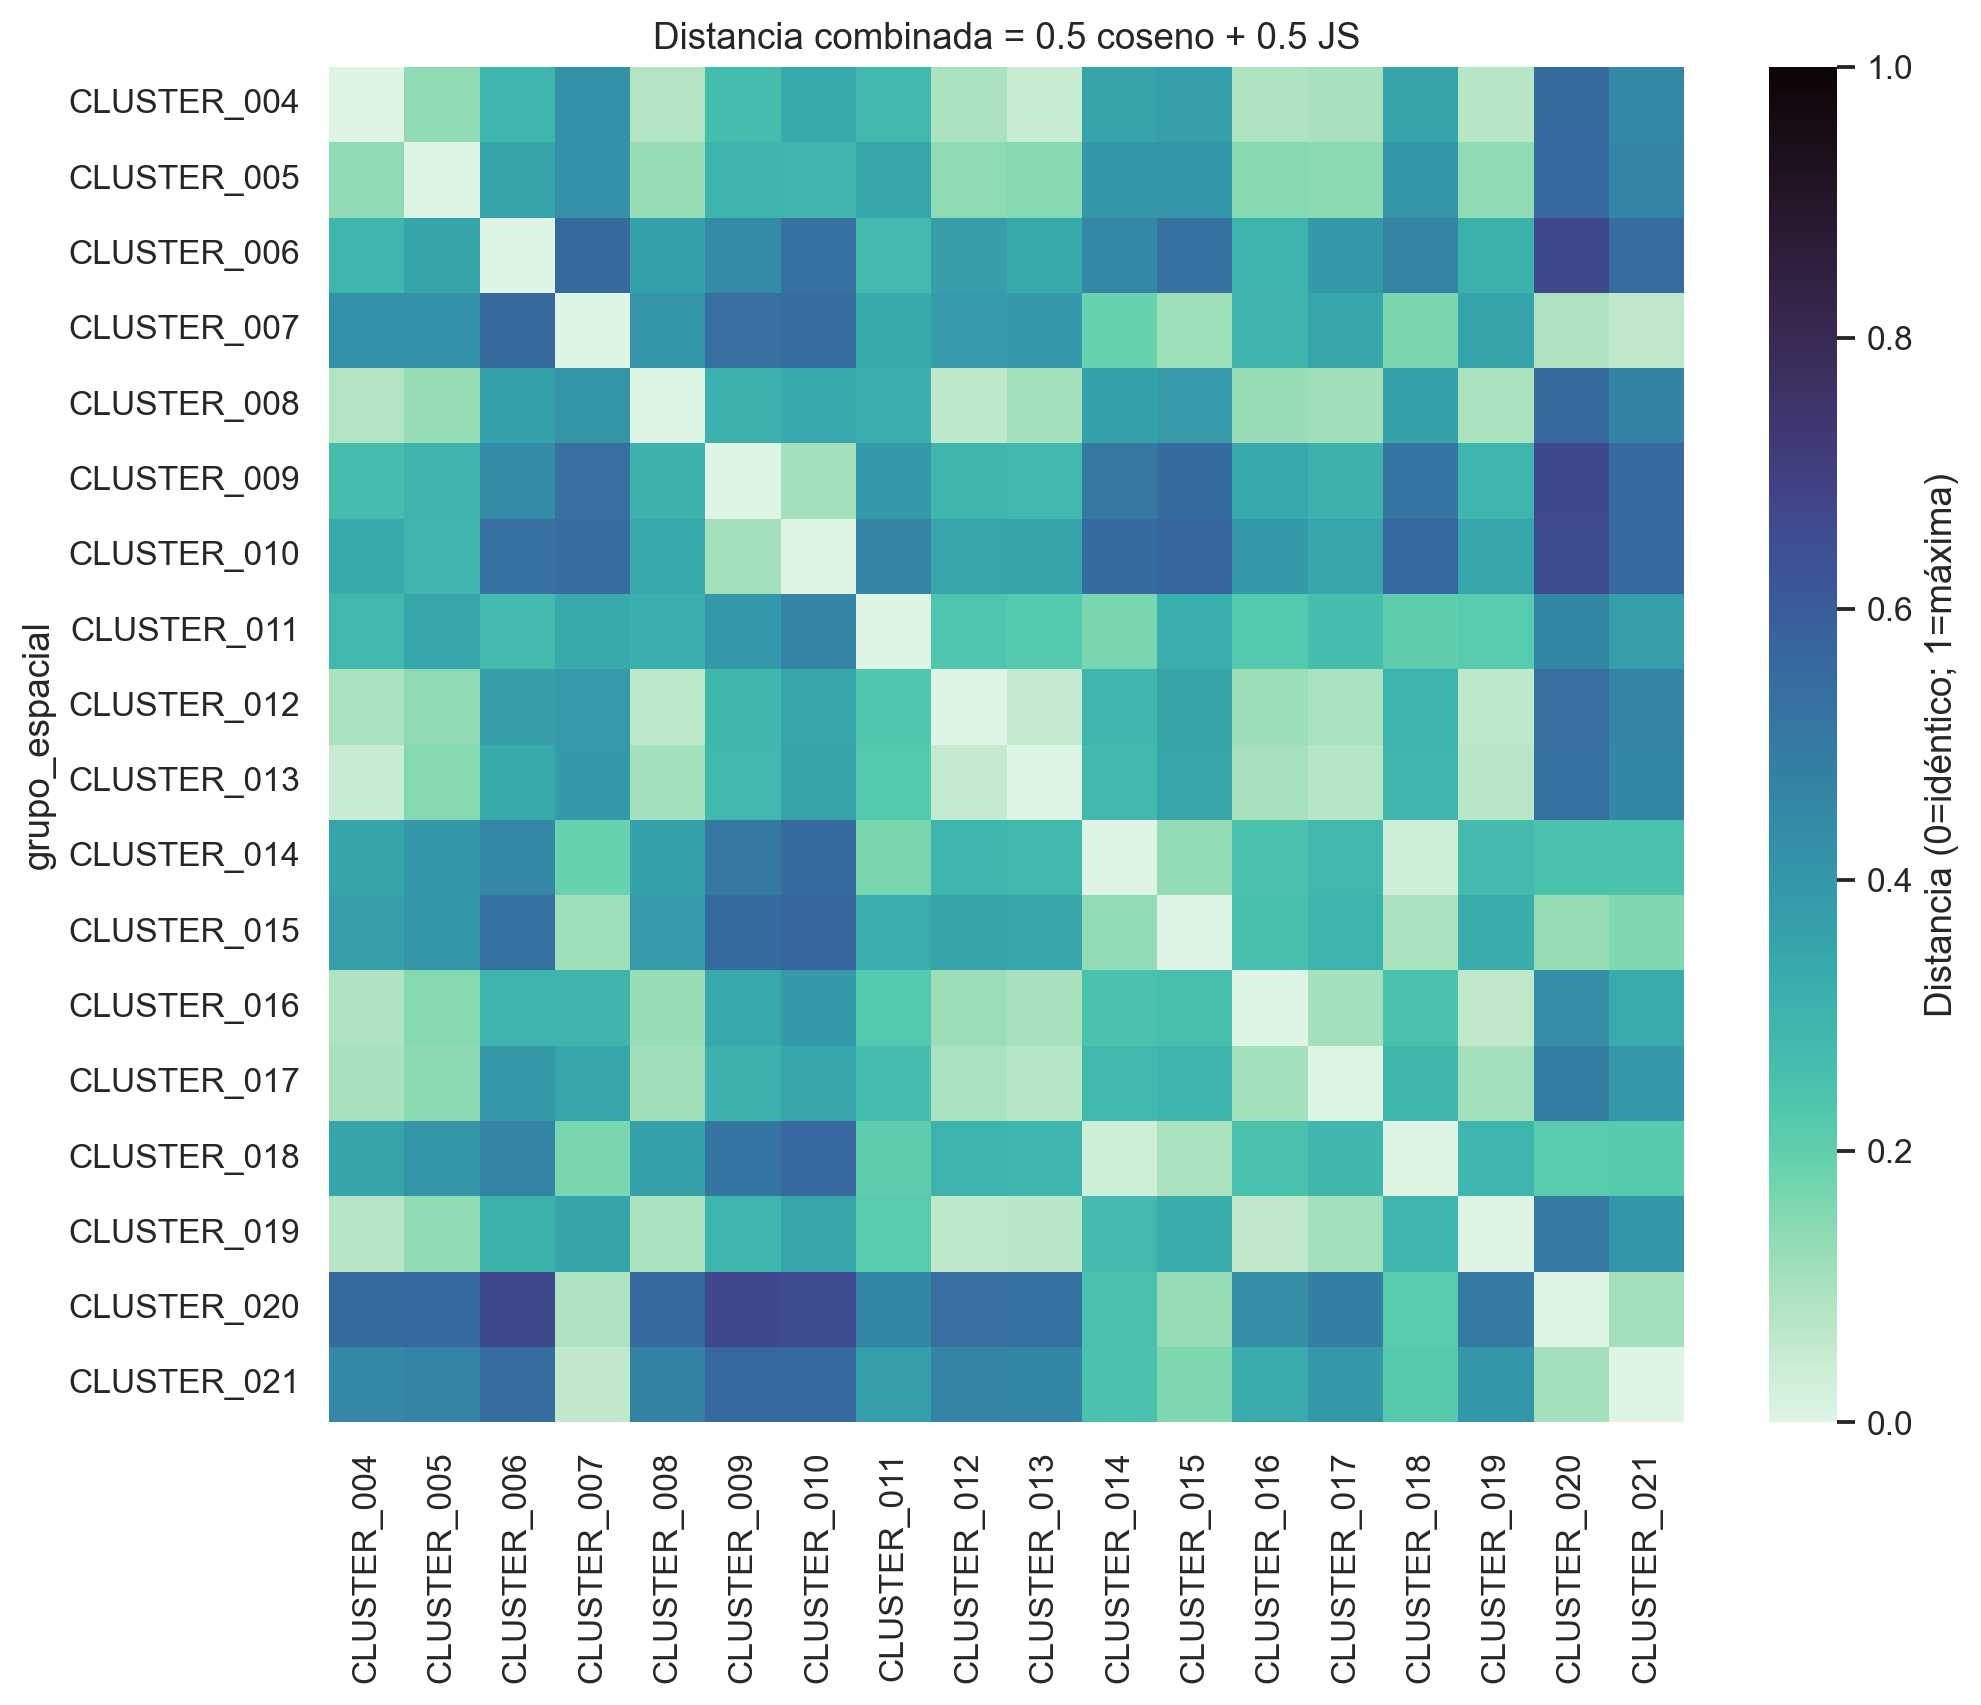
\includegraphics[height=.88\paperheight]{06_distancia_combinada_50_50.png}\end{frame}
\begin{frame}[plain]\centering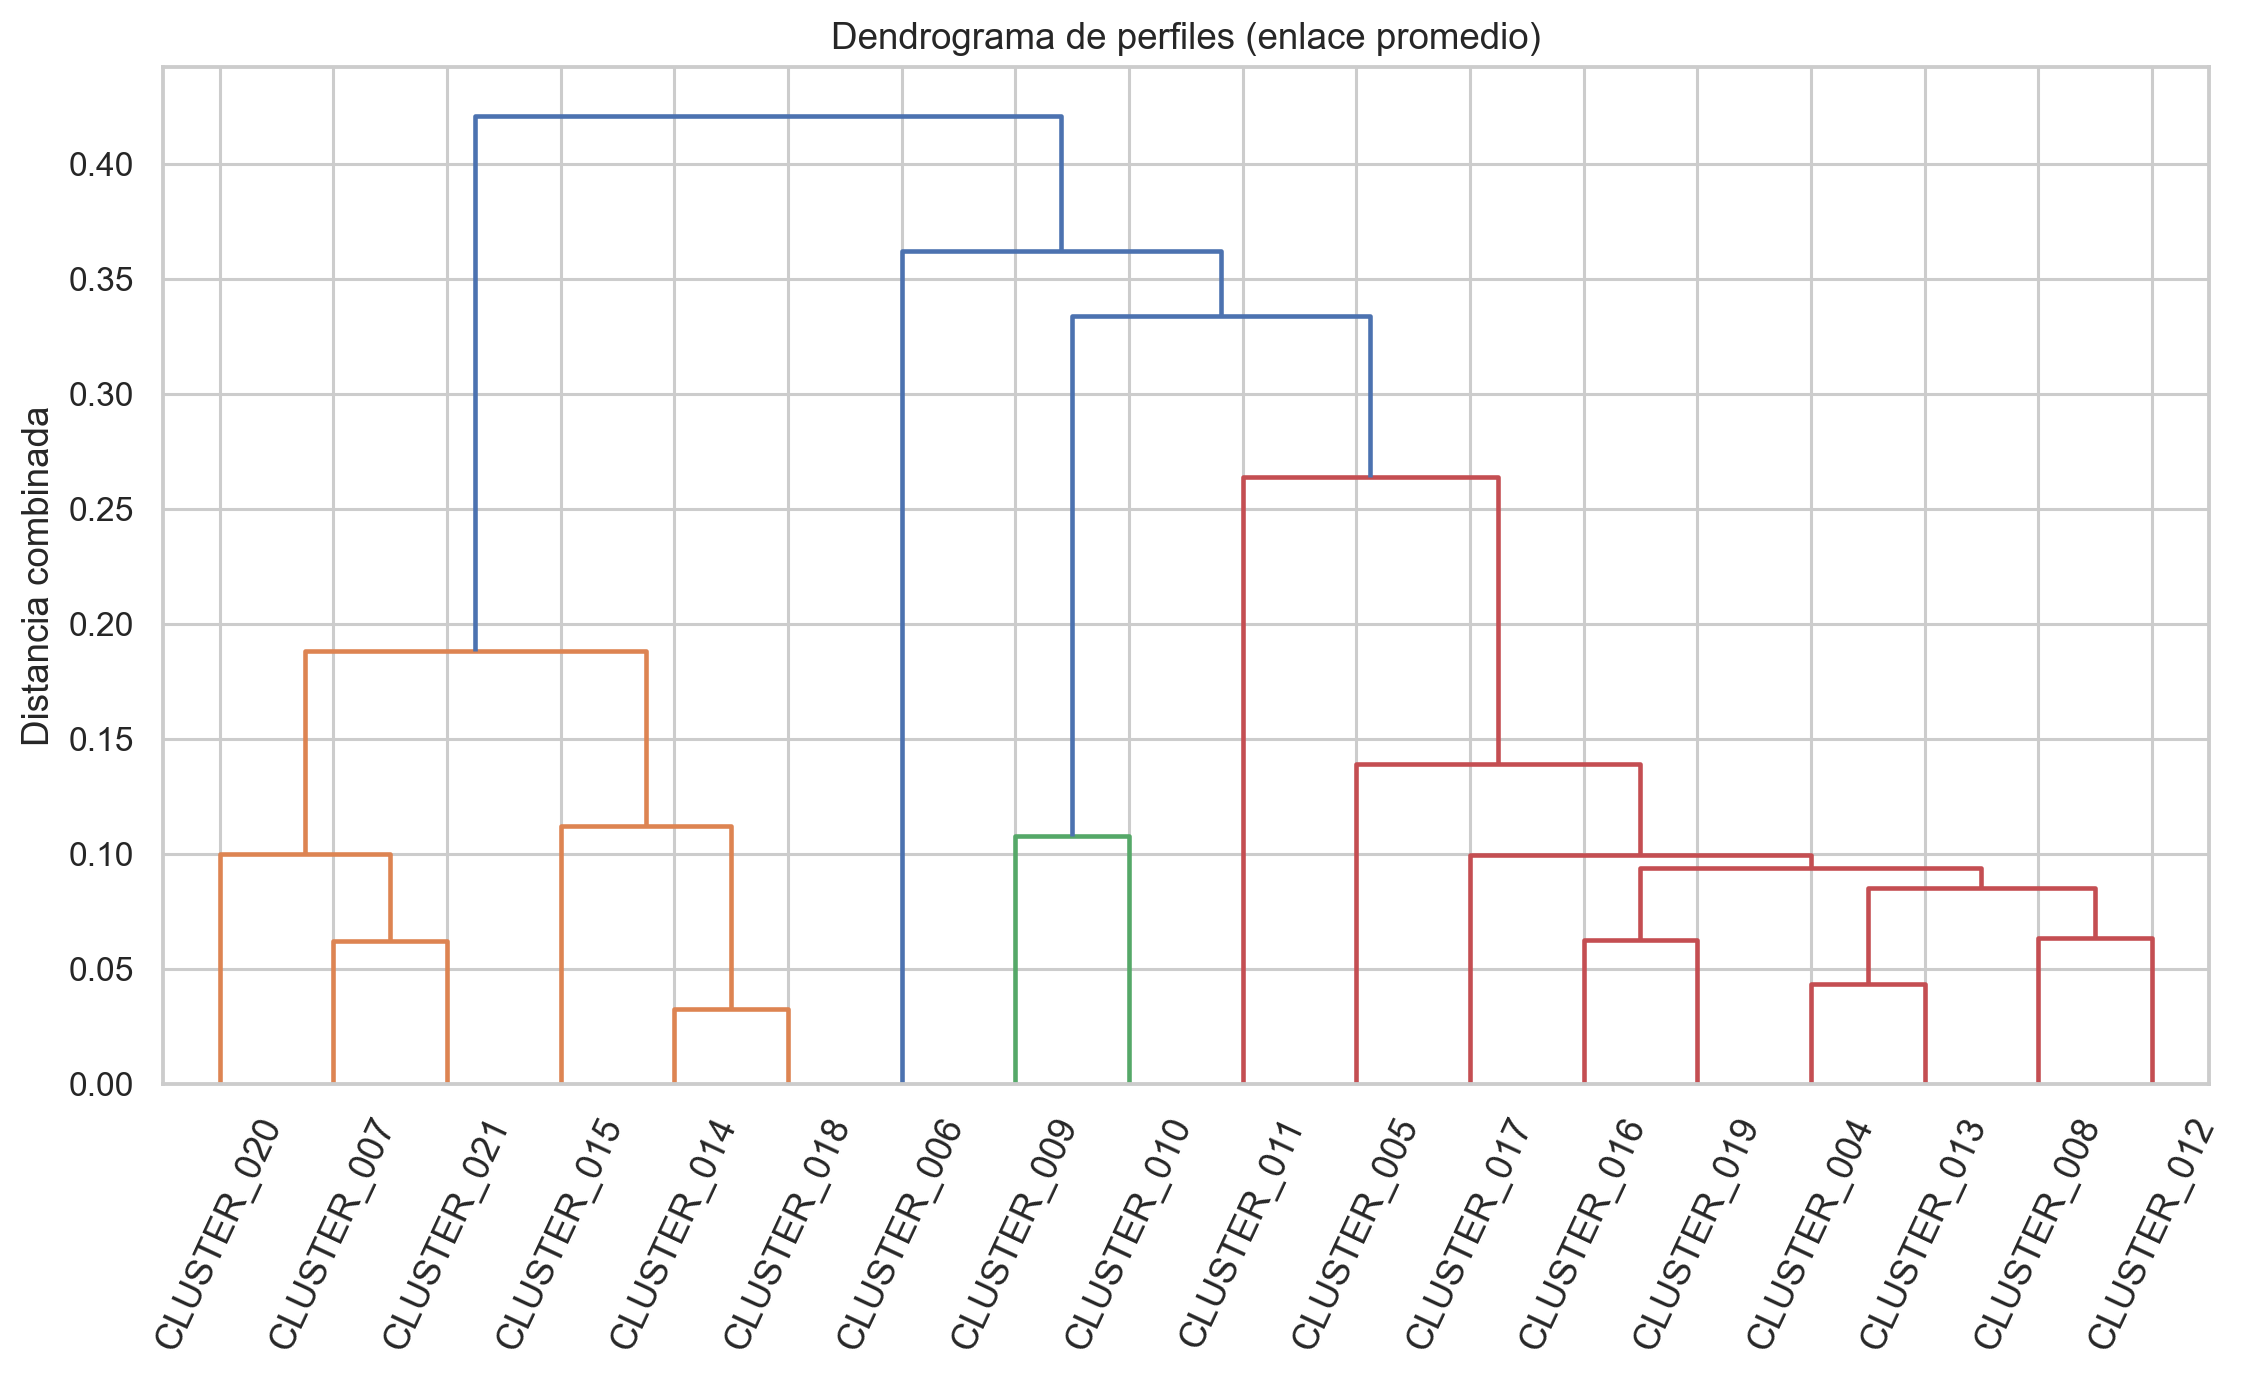
\includegraphics[width=.90\paperwidth,height=.84\paperheight,keepaspectratio]{07_dendrograma_perfiles.png}\end{frame}
\begin{frame}{Pares más próximos}14--18 (0.029), 4--13 (0.042), 12--13 (0.045), 16--19 (0.055), 7--21 (0.055). El reporte enumera señales y SCIAN compartidos y las diferencias que aún los separan.\end{frame}
\begin{frame}{Actividad dispersa}578 establecimientos interiores. ``Ruido'' depende de escala y parámetros; no significa ausencia de actividad ni forma un cluster comparable.\end{frame}
\begin{frame}{Entrega interactiva}HTML autocontenido: selección y comparación de clusters, conteos/porcentajes, señales presentes, etiquetas compactas/ampliadas, SCIAN, sobre-representación, estabilidad, probabilidad y borde.\end{frame}
\begin{frame}{Conclusiones}La estructura combina un continuo metropolitano, concentraciones menores y actividad dispersa. La solución es estable, aunque el ARI global se beneficia del mega-cluster. Las lavanderías aparecen en estructuras mixtas, no casi exclusivas. Parte 3 estudiará hidrología sin retroalimentar el clustering.\end{frame}
\begin{frame}{Límites}DENUE no mide procesos ni descargas. Multilabel no es clasificación exclusiva. Distancia productiva no es distancia geográfica. Asociación espacial no prueba relación empresarial, hidráulica ni causal.\end{frame}\end{document}